\chapter{Bases e Pseudopotenciais\label{apd:bases}}
O método de Auto Consistência aplicado à Hartree-Fock e à Teoria do Funcional da Densidade requer uma Função de Onda \textit{teste} $ \Psi_t $. De acordo com o Postulado \ref{post_anti} essa função de onda desconhecida pode ser descrita como uma combinação linear antissimétrica dos orbitais de um elétron $ \varphi_i $. Desse modo, é possível expandir os orbitais atômicos de uma função de onda desconhecida em termos de um \textit{conjunto de bases} localizadas no orbital atômico e dadas por expressões conhecidas. 

Dessa maneira, na Seção \ref{base} será apresentado os principais conceitos que garantem a validade e a convergência dessa expansão e nas Seções \ref{sto} e \ref{gto} serão abordados as principais bases de átomo centrada utilizados nos cálculos de DFT.

\section{Bases\label{base}}
De acordo com os postulados da Mecânica Quântica, a função de onda $ \Psi $ que descreve um sistema quântico pertence ao espaço de Hilbert. Assim, para expandir a função de onda teste $ \Psi_t $ em termos de um conjunto de bases conhecidas, é necessário que esse conjunto de funções seja \textit{completo} e \textit{ortonormal}. Além disso, a convergência da expansão de $ \Psi_t $ é assegurada a menos que, esse conjunto seja \textit{fechado}.

\begin{mydef}[Sequência de Cauchy]
	Uma sequência $ \Bqty{a_n}_{n\in\mathbb{N}} $ é dita de \textit{Cauchy} se dado $ \epsilon>0 $, existe $ n_{0} \in \mathbb{N} $ tal que para todo $ m,n>n_{0}$ tem-se $ \abs{a_n-a_m}<\epsilon $.
\end{mydef}
\begin{mydef}[Espaço de Hilbert]
	O Espaço de Hilbert é um Espaço Vetorial normado munido de produto interno, no qual toda \textit{Sequência de Cauchy} converge.
\end{mydef}

Nesse sentido, um conjunto de funções ortonormais $ \Bqty{f_i(x)} $ é dito \textit{completo}, se toda função $ g(x) $ no espaço de Hilbert pode ser expressa como combinação linear de $ f_i(x) $.
\begin{mydef}[Conjunto Completo Ortonormal]
	Seja $ g(x) $ uma função no Espaço de Hilbert e $ \Bqty{f_i(x)} $ um conjunto ortonormal de funções. Se a sequência de somas parciais $ g_n(x)\equiv\sum_{i=1}^{n}a_if_i(x) $ converge na média para $ g(x) $, então $ \Bqty{f_i(x)} $ é um conjunto completo ortonormal.
	\begin{equation}
		g(x)\doteq\sum_{i=1}^{\infty} a_if_i(x)
	\end{equation}
\end{mydef}
\begin{mydef}[Conjunto Fechado Ortonormal]
	Um conjunto de funções ortonormais $ \Bqty{f_i(x)} $ é fechado se, a única função ortonormal a toda função de tal conjunto é a função identicamente nula, nesse caso $ \Bqty{f_i(x)} $ é uma base para o Espaço de Hilbert.
\end{mydef}
\begin{teo}\label{teo_base}
	Um conjunto de funções ortonormais no Espaço de Hilbert é completo se e somente se, esse conjunto é fechado.
\end{teo}
\begin{proof}
	A prova do Teorema \ref{teo_base} pode ser encontrada em \cite[Cap. 5,p. 222]{byron} 
\end{proof}

Considerando que a função de Onda $ \Psi $ é descrita no Espaço de Hilbert, então pode ser expandida numa base completa. No entanto, para os cálculos computacionais, escolhe-se um conjunto de bases limitado, uma vez que quanto maior maior o número de bases, maior o custo computacional.

Assim, considerando a equação de Kohn-Sham dada por:
\begin{equation}\label{eq:base_eq1}
	\bqty{-\frac{1}{2}\laplacian+V_H(\vb{r})+w(\vb{r})+v_{xc}(\vb{r})}\orbital=\varepsilon_i\orbital
\end{equation}

O termo entre parênteses é denominada\textit{ Hamiltoniana das equações de Kohn-Sham}. A equação acima é aplicada de modo semelhante para o formalismo de Hartree-Fock, onde o potencial de \textit{Troca e Correlação} $ v_{xc} $ é trocado pelo potencial de \textit{Troca} $ v_x $ \cite{book_HF_2}.

Expandindo o orbital $ \orbital $ sobre um conjunto de bases $ \chi $ de tamanho Q suficientemente maior que o número de estados ocupados N.
\begin{equation}
	\orbital=\sum_{p=1}^{Q} C_{ip}\chi_p(\vb{x})
\end{equation}

Reescrevendo a equação \eqref{eq:base_eq1} em termos de um operador Hamiltoniano $ \mathcal{H} $ e multiplicando-se pela base conjugada $ \chi^\ast $, tem-se:
\begin{equation}\label{eq:base_eq2}
	\sum_p C_{ip}\bqty{\int\baseconj\mathcal{H}\base\dd\vb{x}-\varepsilon_i\int \baseconj\base \dd{\vb{x}}}=0
\end{equation}

A equação acima é um sistema de equações algébricas. A matriz dos elementos (matriz de \textit{overlap}) da base $ S_{qp}$ precisa ser calculada uma única vez e é definida como:
\begin{equation}
	S_{qp}\equiv \int \baseconj\base \dd{\vb{x}}
\end{equation}

A matriz de elementos do operador Hamiltoniano corresponde a:
\begin{equation}\label{eq:matriz_halm}
	H_{qp}\equiv\int\baseconj\bqty{-\frac{1}{2}\laplacian+V_H(\vb{r})+w(\vb{r})+v_{xc}(\vb{r})}\base \dd{\vb{x}}
\end{equation}

E depende dos coeficiente desconhecidos $ C_{ip} $ através de $ \rho $ e $ v_{xc} $. Por outro lado, a dependência dos coeficientes por meio do $ \rho $ pode ser simplificada da seguinte forma:
\begin{equation}
	\densx=\sum_{i=1}^{N} \orbitalconj \orbital =\sum_{pq}\underbrace{\bqty{\sum_{i=1}^{N}C_{iq}^{\ast}C_{ip}}}_{\equiv D_{pq}}\baseconj\base
\end{equation}

Portanto, a dependência da matriz $ H_{qp} $ dos coeficientes $ C_{iq} $ é determinada pela \textit{Matriz Densidade} $ D_{pq} $, de modo que é possível aplicar o análogo do método de auto consistência para a matriz densidade. Dessa forma, fixando-se um conjunto de coeficientes testes na matriz densidade, constrói-se a matriz do operador Hamiltoniano, equação \eqref{eq:matriz_halm}, de maneira que a equação \eqref{eq:base_eq2} resulta em um sistema de equações lineares resolvida por diagonalização. O processo se repete até a matriz densidade convergir de acordo com o critério de auto consistência descrito abaixo e ilustrado pela figura \ref{fig:criterio}. 
\begin{equation}
	C^{next}=\beta C^{new}+(1-\beta)C^{old} \qquad \beta<1
\end{equation}
\begin{figure}[H]
	\centering
	\caption{Esquema ilustrativo do método de auto consistência usado para a matriz densidade. O esquema mostra a dependência entre a solução de saída ($ C^{out} $) e a solução de entrada ($ C^{in} $). A reta tracejada representa a condição de auto consistência.}
	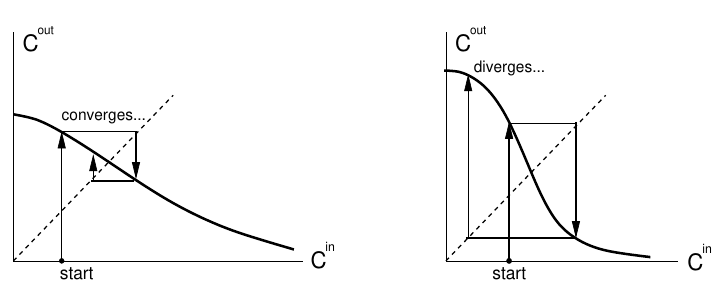
\includegraphics[scale=0.6]{figs/criterio.png}
	\legend{Fonte: \citeauthor{book_base}}
	\label{fig:criterio}
\end{figure}

Quando o sistema apresenta condições de contorno periódicas tais como sólidos, utiliza-se uma base que não depende das posições atômicas como a base \textit{"Ondas Planas"}. De modo geral, a expansão em Ondas Planas pode ser descrita da seguinte maneira:
\begin{equation}
	\varphi_i(\vb{r})=\frac{1}{\sqrt{\Omega}}\exp\bqty{i G_i\cdot \vb{r}}
\end{equation}

Por outro lado, ao realizar a expansão do orbital sobre um conjunto de funções de bases conhecidas, é possível realizar essa expansão de modo que essa base seja centrada em algum ponto do espaço. Para sistemas não periódicos, como moléculas, utiliza-se normalmente as bases centrada no núcleo denominada \textit{"Átomo-Centrada"}. As principais bases de átomo centrada são as bases \textit{Orbital do Tipo Slater} e \textit{Orbital do Tipo Gaussiana}. \cite{book_base}


\subsection{Orbital do Tipo Slater (STO)\label{sto}}

O conjunto de bases de átomo-centrada denominada \textit{Orbital do Tipo Slater} foi introduzida em 1930 pelo físico John C. Slater \cite{base_slater} e baseia-se na função de onda do átomo de hidrogênio, tendo sua forma dada por:
\begin{equation}
	\chi_{STO}(\vb{r}) = N r^{n-1}e^{\zeta r}\mathrm{Y}_{l,m}(\theta,\phi) \qquad n\in \mathbb{N}
\end{equation}

Onde \textit{r} é a distância dos elétrons ao núcleo atômico, \textit{n} representa o número quântico principal, $ \zeta $ é um parâmetro ajustável que representa a carga nuclear efetiva e \textit{N} é um fator de normalização. As bases do tipo STO formam um base de solução completa.

Uma característica dessa base é que ela não permite a estrutura de \textit{nós} assim como a solução do átomo de hidrogênio. Para permitir a estrutura de nós através dessa base é necessário uma combinação de várias bases STO. Nesse sentido, surge o conceito de \textit{Base Mínima}, ou seja a representação mais simples possível de um orbital atômico, como pode ser observado na Tabela . A base mínima contém uma função de base para cada orbital ocupado. Por outro lado, variando-se os valores do parâmetro $ \zeta $ é possível expandir a base mínima, de modo que essa nova base estendida é denominada "Duplo-Zeta", "Triplo-Zeta", etc. 
\begin{table}[H]
	\centering
	\caption{Tabela mostrando os orbitais dos elementos da tabela periódia em termos da Base Mínima e da Base Duplo-Zeta.}
	\begin{tabular}{ccc} 
		\hline\hline
		& Base Mínima         & Duplo-Zeta                  \\ \hline
		H, He               & 1s                  & 1s, 1s'                     \\
		Li $\rightarrow $ Ne & 1s, 2s, 2p          & 1s, 1s', 2s, 2s', 2p, 2p'   \\
		Na $\rightarrow $ Ar & 1s,$\ldots$, 3p, 3d & 1s, 1s', $\ldots$, 3d, 3d'  \\
		K $\rightarrow $ Kr  & 1s,$\ldots$, 4s, 4p & 1s, 1s',$\ldots$, 4p, 4p'   \\
		Rb $\rightarrow $ Xe & 1s,$\ldots$, 5s, 5p & 1s, 1s',$\ldots$, 5p, 5p'   \\
		\hline\hline
	\end{tabular}
	\legend{Fonte: \citeauthor{book_base}}
	\label{tab:base_minima}
\end{table}
A base STO converge rapidamente para o resultado quando aumenta-se o número de bases. No entanto, as integrais que envolvem a base STO são difíceis de resolver.
%
%\subsection{Orbital do Tipo Gaussiana (GTO)\label{gto}}
%
%A conjunto de bases denominada \textit{Orbital do Tipo Gaussiana} foi proposta em 1950 por Boys \cite{base_gauss}, sendo representada por:
%\begin{equation}
%	\chi_{GTO}= N r^{2(n-1)}e^{-\zeta r^2}\mathrm{Y}_{l,m}(\theta,\phi) \qquad n\in \mathbb{N}
%\end{equation}
%
%A base do tipo Gaussiana se destaca pela possibilidade de calcular as integrais analiticamente. A base GTO impõe uma restrição sobre as bases usadas, de modo que somente as funções de onda que obedeçam a $ l=n-1 $ são usadas, ou seja, 1s, 2p, 3d, $ \ldots$, mas não 2s, 3p, $\ldots  $ O conjunto de bases STO possui uma convergência melhor que o conjunto de bases GTO, uma vez que a GTO não representa de forma correta os comportamentos assintóticos da função de onda do um elétron, como pode ser observado na Figura \ref{fig:gto1} para o orbital 1s do átomo de hidrogênio. Por outro lado, é possível representar uma STO com uma combinação linear de GTO's, como mostra a Figura \ref{fig:gto2} no qual aproximou-se o orbital 1s por uma combinação linear de GTO.
%
%
%%
%%\begin{figure}[H]
%%	\centering
%%\subfig[Utilizando uma base GTO. Fonte: \cite{book_base}]{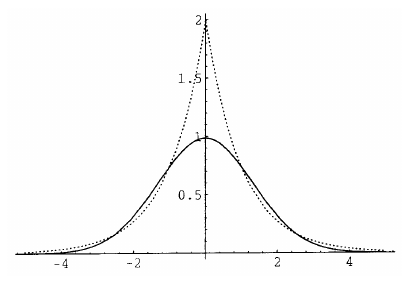
\includegraphics[scale=0.65]{figs/gtoh1.png}\label{fig:gto1}} \qquad
%%\subfig[Representação através de uma combinação linear de GTO's. Fonte: \cite{book_base}.]{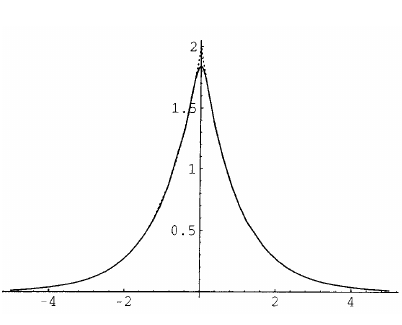
\includegraphics[scale=0.65]{figs/gto1sh1.png}\label{fig:gto2}}
%%	\caption{\textit{Representação do orbital 1s do átomo de hidrogênio (linha pontilhada) através da base GTO (linha contínua).}}
%%\end{figure}
%
%\begin{figure}[H]
%	\centering
%	\begin{subfigure}[b]{0.45\textwidth}            
%		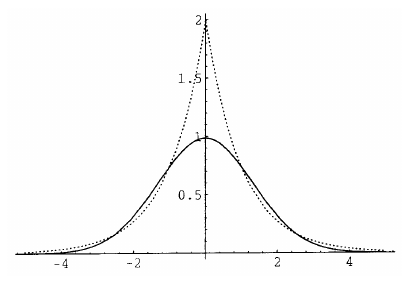
\includegraphics[width=\textwidth]{figs/gtoh1.png}
%		\caption{\textit{Representação usando uma base GTO. Fonte: \cite{book_base}}}
%		\label{fig:gto1}
%	\end{subfigure} \quad%
%	%add desired spacing between images, e. g. ~, \quad, \qquad etc.
%	%(or a blank line to force the subfigure onto a new line)
%	\begin{subfigure}[b]{0.37\textwidth}
%		\centering
%		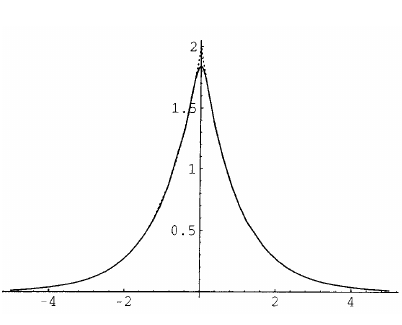
\includegraphics[width=\textwidth]{figs/gto1sh1.png}
%		\caption{\textit{Representação através de uma combinação linear de GTO's. Fonte: \cite{book_base}.}}
%		\label{fig:gto2}
%	\end{subfigure}
%	\caption{\textit{Representação do orbital 1s do átomo de hidrogênio (linha pontilhada) através da base GTO (linha contínua).}}\label{fig:gto}
%\end{figure}
\subsection{Orbital Atômico Numérico (NAO)}
Uma base atômica numérica- Numerical Atomic Orbital (NAO)-  é uma base estendida e localizada que reproduz a base minimal de forma continua, suave e diferenciável a partir de um raio de corte $r_m$. Essa base é representada por:
\begin{equation}
    \chi_{NAO}^I(\vb{r}_I)=\mathcal{R}^I_{nl}(r_I)\mathrm{Y}_{l,m}(\theta,\phi)
\end{equation}
onde, para cada átomo I, $\mathcal{R}^I_{nl}(r_I)$ é a função radial do n-ésimo orbital. 

A suavidade e o ajuste dessa base são definidos por um deslocamento de energia $\delta \epsilon$ (\textit{Energy Shift})  ganho devido ao confinamento dos orbitais em bases localizadas. Essa base apresenta uma melhor convergência com menos bases estendidas e corresponde ao tipo de base utilizada no código \textit{Siesta} \cite{nao}.

\section{Pseudopotenciais}

Devido à complexidade e ao custo computacional em um cálculo de muitos elétrons, é necessário utilizar aproximações que permitem modelar tais sistemas. Nesse sentido, o \textit{Método de Pseudopotencial} constitui uma importante ferramenta na otimização do custo computacional, uma vez que, substitui os efeitos dos elétrons do caroço por um potencial efetivo. Assim, nesse capítulo será apresentado os principais requisitos de um pseudopotencial.

O \textit{Método de Pseudopotencial}consiste em substituir os efeitos devido aos elétrons do caroço por um potencial efetivo, de modo a tratar somente os elétrons de valência. Os elétrons do caroço são aqueles mais próximos ao núcleo que não participam das ligações químicas. Assim, as propriedades químicas e físicas importantes em moléculas e materiais são determinadas pelos elétrons de valência \cite{tese_pseudo}. Nesse sentido, os estados dos elétrons do caroço são considerados como \textit{inertes}, de modo que através de um cálculo \textit{atômico} com todos os elétrons, obtém-se a forma espacial dos elétrons do caroço e considera-se que a função de onda dos elétrons do caroço permanece a mesma tanto para cálculos de moléculas, quanto para sólidos. A vantagem de substituir o potencial do núcleo por um potencial gerado pelo caroço reside no fato de que esse último é mais suave \cite{book_base}

A ideia de substituir o átomo por um caroço iônico que interage com os elétrons de valência, foi proposta inicialmente por E. Fermi em 1934 \cite{fermi}. Em 1935, Hellmann sugeriu a expressão abaixo para representar o potencial sentido pelos elétrons de valência do Potássio \cite{fermi_2}.
\begin{equation}
	w(r)=-\frac{1}{r}+\frac{274}{r}e^{-1.16r }
\end{equation}

No entanto, somente em 1959 com as contribuições de Phillips e Kleinman que os pseudopotenciais começaram a ser largamente utilizados \cite{pseudo_ref}. Com o advento e os avanços da Teoria do Funcional da Densidade, os pseudopotenciais passaram a ser gerados a partir da solução das Equações de Kohn-Sham para o problema atômico envolvendo todos os elétrons. \cite{toffoli_pseudo}

A construção de um pseudopotencial inicia com a escolha apropriada da configuração eletrônica do átomo, denominada \textit{configuração de referência}. Nessa etapa, separa-se na distribuição das camadas eletrônicas os elétrons do caroço e os elétrons de valência, além disso, acrescenta-se estados vazios aos estados dos elétrons de valência, a fim de incluir configurações iônicas. Outro requisito é que, a partir do ponto denominado \textit{Raio de Corte} $ r_c $, a função de onda de valência devido ao pseudopotencial seja igual a função de onda de valência obtida no cálculo com todos os elétrons \cite{book_base}. 

Na Figura \ref{fig:pseudo} está ilustrado o exemplo de um gráfico da função de onda em função do raio de corte para cada  valor do número quântico \textit{l} de uma determinada configuração iônica. Além disso, no gráfico está representado a função de onda correspondente ao cálculo com todos os elétrons realizados utilizando o funcional vdw-DF1 \cite{DRSLL}. Além disso, está representada a diferença existente entre os pseudopotenciais gerados pelo funcional GGA-PBE (\textit{PS-pbe}) e o funcional vdw-DF1 (\textit{PS-vdw}), junto aos respectivos raios de corte utilizados $ R_{pbe} $ e $ R_{vdw} $.
\begin{figure}[]
	\centering
	\caption{Gráfico da Função de Onda dos elétrons de valência da configuração de referência usada para o Paládio, calculados usando o funcional VDW-DRSLL e o funcional PBE. No gráfico está o cálculo com todos os elétrons e com o pseudopotencial em função do Raio.}	\label{fig:pseudo}
	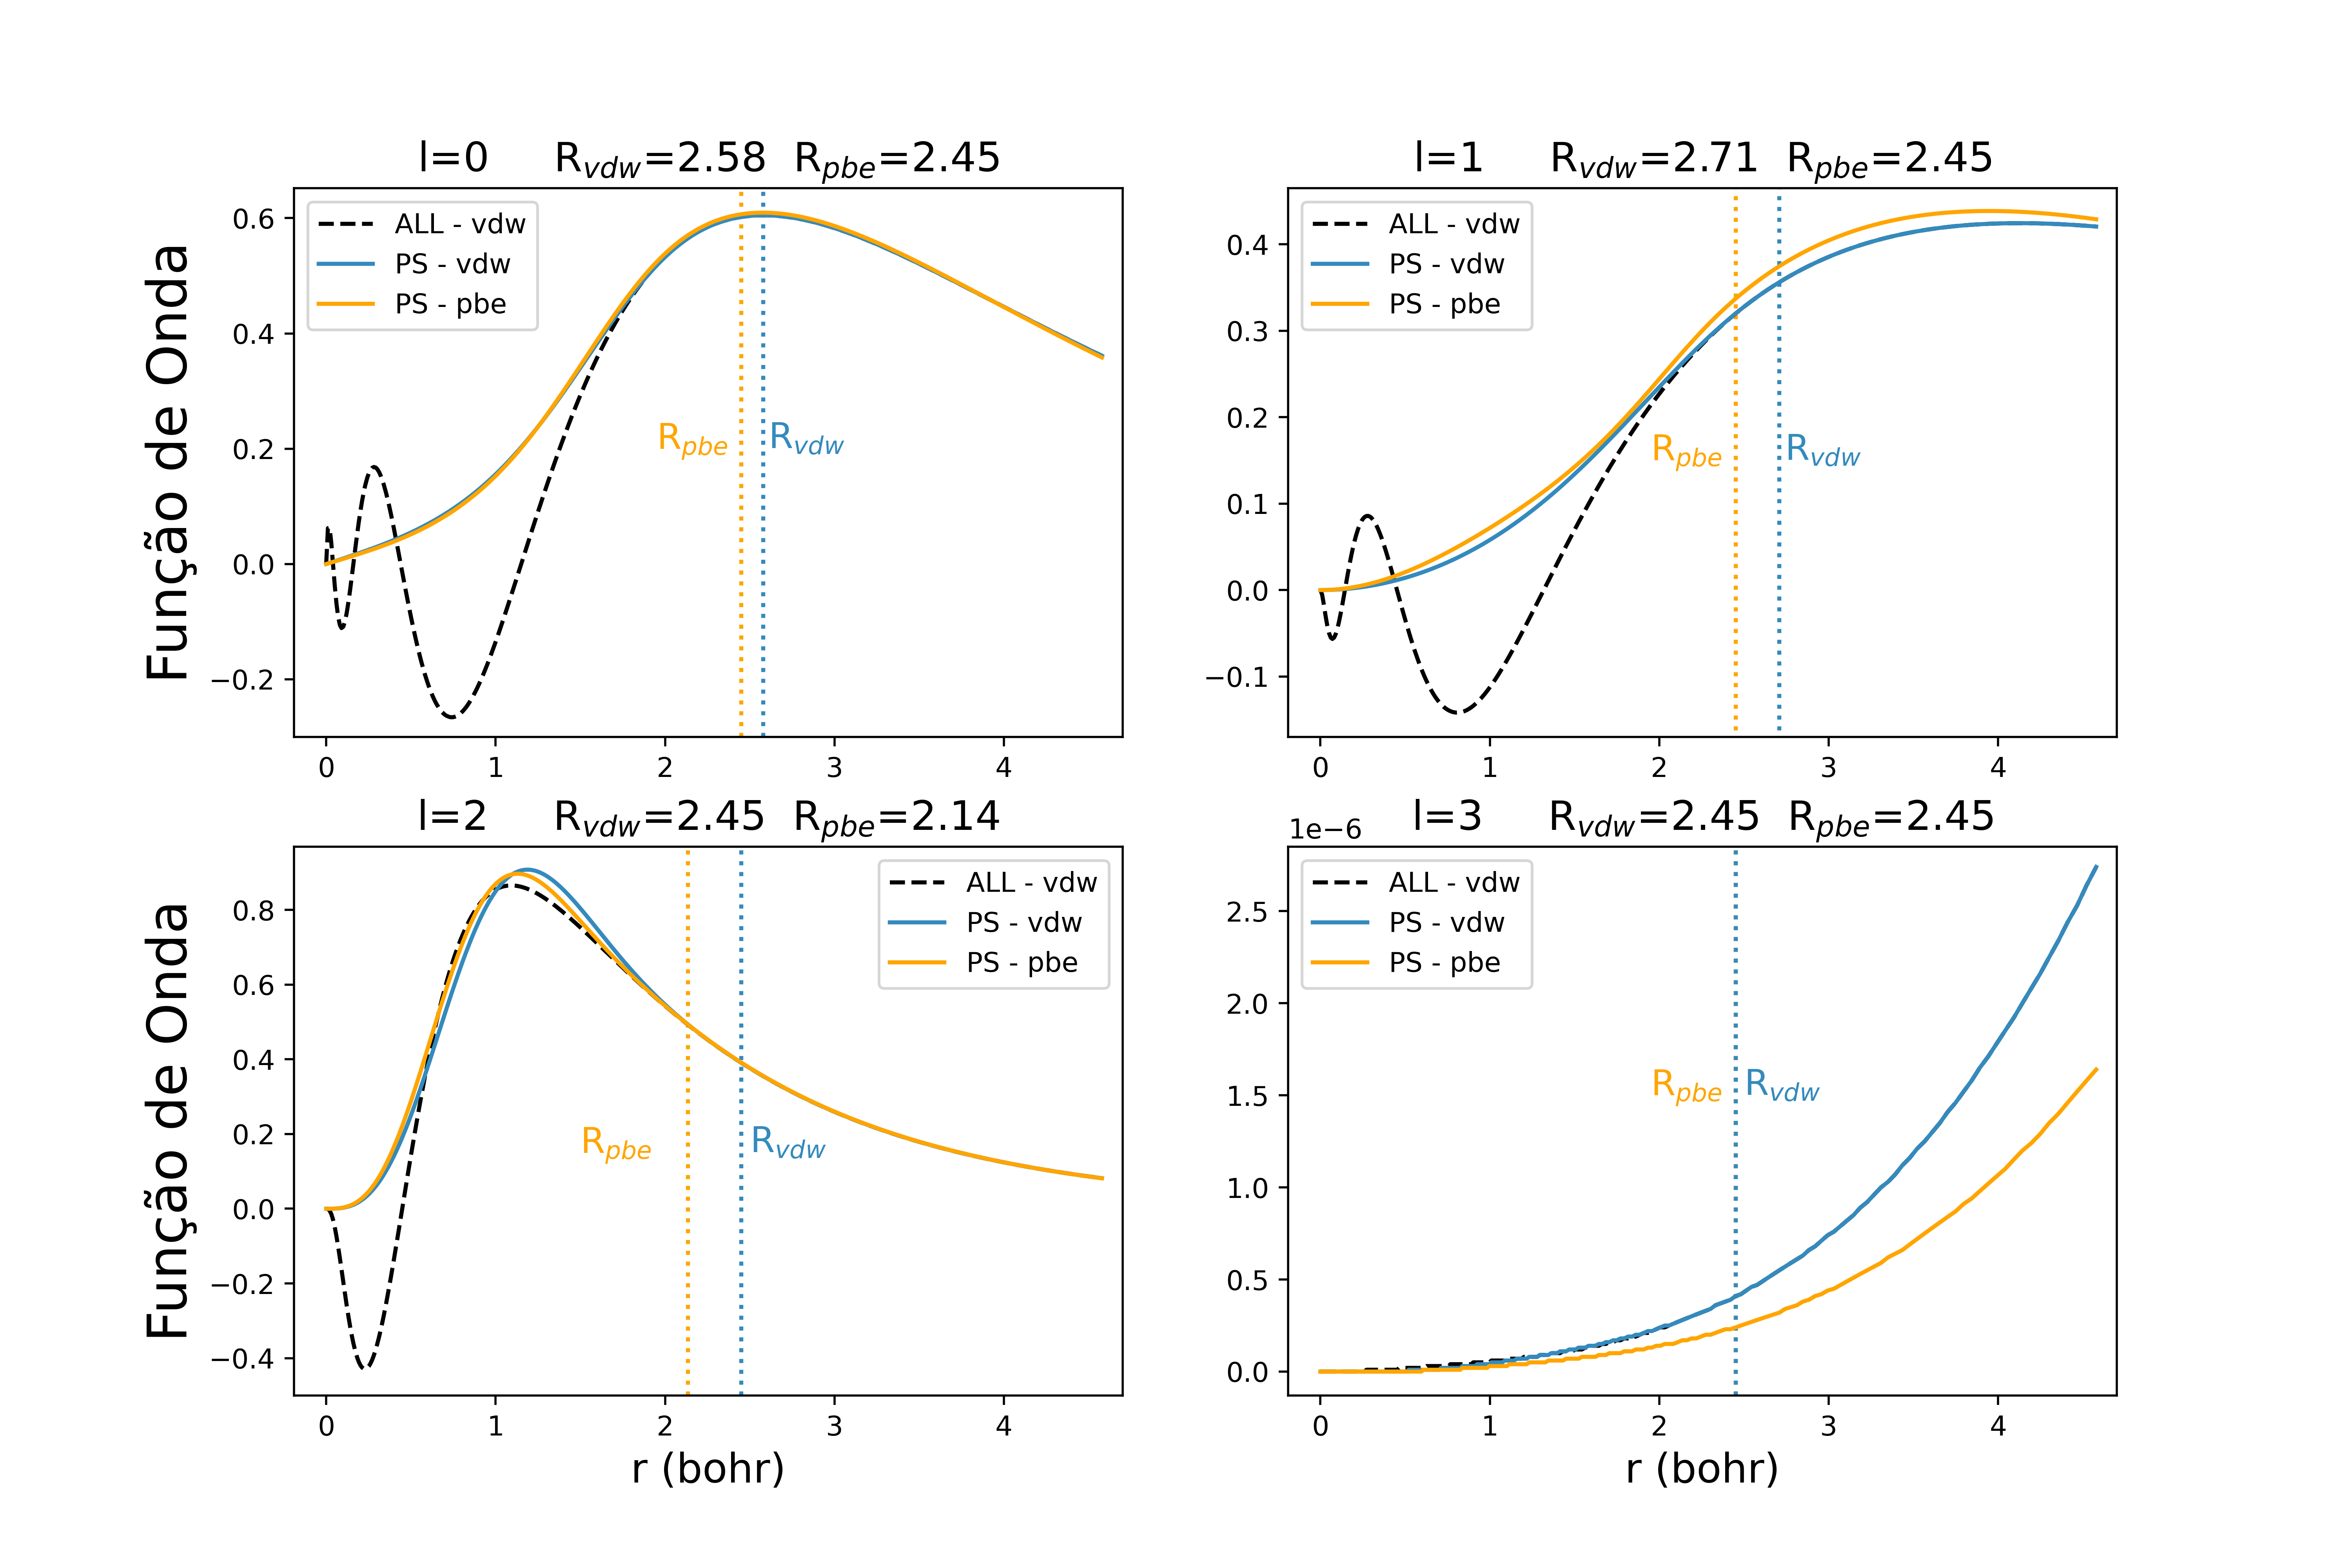
\includegraphics[scale=0.45]{figs/pseudo.png}
\legend{Fonte: Compilação da autora.}
\end{figure} 

Para encontrar as pseudofunções $ \varphi^{PS} $ geradas a partir do pseudopotencial, considere que as autofunções $ \Psi $ da Hamiltoniana $ \hat{H} $ é dada pela soma das autofunções do caroço $ \ket{\varphi_{c}} $ e de valência $ \ket{\varphi_{v}} $, tal que:
\begin{eqnarray}
	\hat{H}\ket{\psi_{c}}&=&\varepsilon_{c}\ket{\psi_{c}}\label{eq:caroco}\\
	\hat{H}\ket{\psi_{v}}&=&\varepsilon_{v}\ket{\psi_{v}}\label{eq:valencia}
\end{eqnarray}
Onde, foi utilizada a notação vetorial de Dirac. 

Supondo que a autofunção que corresponde ao pseudopotencial tem que ser uma função suave, então ela pode ser escrita em termos dos estados de valência $ \ket{\psi_{v}} $ e em termos da ortogonalização entre as autofunções de valência e as autofunções do caroço, tem-se:
%Supondo que, os orbitais de valência $ \ket{\psi_{v}} $ podem ser escritos em termos de uma função mais suave $ \ket{\varphi_v^{PS}} $, a função de onda gerada pelo pseudopotencial, somada à expansão dos orbitais de valência na base dos orbitais do caroço, tem-se a expressão abaixo \cite{pseudo_ref}.
\begin{equation}
	\ket{\varphi_v^{PS}}=\ket{\psi_{v}}+\sum_{c} \alpha_{cv}\ket{\psi_c}
\end{equation}
Onde,
\begin{equation}
	\alpha_{cv}=\braket{\psi_c}{\varphi_v^{PS}}
\end{equation}


Multiplicando por uma autofunção do caroço  $ \ket{\psi_{c'}} $ e integrando obtém-se os coeficientes $ \alpha_{cv} $:
\begin{equation}
	\braket{\psi_{c'}}{\varphi_v^{PS}}=\underbrace{\braket{\psi_{c'}}{\psi_{v}}}_{\substack{\text{= 0,}\\ \text{pois os estados de} \\ \text{valência e do}\\ \text{caroço pertencem} \\ \text{á mesma} \\ \text{Hamiltoniana}}}+\sum_{c}\alpha_{cv}\underbrace{\braket{\psi_{c'}}{\psi_{c}}}_{= \delta_{cc'}}
\end{equation}

A Equação de Schr$\"{o} $dinger para o a função de onda do pseudopotencial $  \ket{\varphi_v^{PS}}$ é dada por:
\begin{eqnarray}
	\hat{H}\ket{\varphi_v^{PS}}&=&\hat{H}\ket{\psi_{v}}+\sum_{c}\alpha_{cv} \hat{H}\ket{\psi_{c}} \\ \nonumber
	&=& \varepsilon_{v}\bqty{\ket{\varphi_v^{PS}}-\sum_{c} \alpha_{cv}\ket{\psi_c}}+\sum_{c} \alpha_{cv}\varepsilon_{c}\ket{\psi_{c}} \\ \nonumber
	&=& \varepsilon_{v}\ket{\varphi_v^{PS}}+\sum_{c}(\varepsilon_{c}-\varepsilon_{v})\alpha_{cv}\ket{\psi_{c}} 
\end{eqnarray}

Como $ \varepsilon_{v} $ é também autovalor de $ \ket{\varphi_v^{PS}} $, então a equação acima resulta em:
\begin{equation}\label{eq:pseudo}
	\bqty{\hat{H}+\sum_{c} (\varepsilon_{c}-\varepsilon_{v})\dyad{\psi_{c}}}\ket{\varphi_v^{PS}}=\epsilon_v\ket{\varphi_v^{PS}}
\end{equation}

Portanto, a \textit{Pseudo-Função de Onda} $ \ket{\varphi_v^{PS}} $ satisfaz a Equação de Schr$ \"{o} $dinger, cuja hamiltoniana é composta pela Hamiltoniana das Equações de Kohn-Sham, somada a uma pseudo-hamiltoniana dependente da energia. O segundo termo da equação \eqref{eq:pseudo} pode ser representado como um potencial repulsivo, pois o pseudopotencial é mais fraco que o potencial real na vizinhança do caroço. Assim reescrevendo a equação \eqref{eq:pseudo} em termos do \textit{Potencial Repulsivo} $ \hat{V}_R $, obtém-se:
\begin{equation}
	\pqty{\hat{H}+\hat{V}_R}\ket{\varphi_v^{PS}}=\epsilon_v\ket{\varphi_v^{PS}}
\end{equation} 

Como resultado, a pseudo função de onda $ \ket{\varphi_v^{PS}} $ satisfaz uma equação com um potencial efetivo $ \hat{V}_{R} $, cujo autovalor é o mesmo da autofunção real de valência $ \ket{\psi_{v}} $, equação \eqref{eq:valencia}. \cite{pseudo_ref}

A fim de obter pseudopotenciais mais suaves e precisos, em 1979 Hamann, Schlüter and Chiang \cite{pseudo_norma} sugeriram quatro critérios a serem cumpridos pelo pseudopontecial na configuração de referência, são as condições de \textit{Norma-Conservada} \cite{toffoli_pseudo}:
\begin{enumerate}
	\item Os autovalores correspondentes às pseudofunções $ \ket{\psi_{nl}^{PS}} $ tem que ser iguais aos autovalores da autofunções com todos os elétrons $ \ket{\psi_{nl}^{AE}} $ para a configuração de referência.
	\begin{eqnarray}
		\hat{H}\ket{\psi_{nl}^{AE}}&=&\varepsilon_{nl}\ket{\psi_{nl}^{AE}} \\ 
		\pqty{\hat{H}+\hat{V}_R}\ket{\psi_{nl}^{PS}}&=&\varepsilon_{nl}\ket{\psi_{nl}^{PS}}
	\end{eqnarray}
	\item As funções de onda do cálculo com todos os elétrons $ \psi_{nl}^{AE} $ tem que ser igual à função de onda gerada pelo pseudopotencial $\psi^{PS}_{nl}(\vb{r})$ a partir do ponto correspondente ao raio de corte $ r_c $.	
	\begin{equation}
		\psi^{AE}_{nl}(r)=\psi^{PS}_{nl}(r) \quad ,\forall \quad r\geq r_c 
	\end{equation}
	\item A densidade de carga da solução de todos os elétrons e para o pseudopotencial integradas no intervalo de 0 a \textit{R} devem ser iguais, para todo $ R\leq r_c $	
	\begin{equation}
		\int_{0}^{R}\abs{\psi^{AE}_{nl}(r)}^{2}r^2 dr=\int_{0}^{R}\abs{\psi^{PS}_{nl}(r)}^{2}r^2 dr
	\end{equation}
	\item A derivada logarítmica e a derivada da energia para ambos os casos tem que ser iguais para todo $ R\leq r_c $
	\begin{equation}
		\bqty{(r\psi^{AE}_{nl}(r))^2\dv{E}\dv{r}\ln \psi^{AE}_{nl}(r) }_{R}=\bqty{(r\psi^{PS}_{nl}(r))^2\dv{E}\dv{r}\ln \psi^{PS}_{nl}(r) }_{R}
	\end{equation}
\end{enumerate}

Em suma, a carga contida dentro do raio de corte é a mesma tanto para o pseudopotencial quanto para o cálculo com todos os elétrons \cite{book_base}.

Dentre as famílias de pseudopotenciais existentes, o pseudopotencial proposto por \textit{Troullier e Martins }\cite{troullier_martins} é um método eficiente, além de apresentar resultados mais suaves. O potencial de Troullier Martins fornece resultados mais precisos para os átomos com estados \textit{2p} de valência da primeira linha da tabela periódica, bem como para estados de valência \textit{d} dos metais de transição \cite{book_base}.

Nesse método, a parte radial da pseudo-funções de onda são definidas por:
\begin{equation}
	R_l^{PS}=\left\{\begin{matrix}
		R_{nl}^{AE}(r) & \text{, se} \quad r>r_c\\ 
		r^{l}e^{p(r)} &\text{, se}\quad r<r_c 
	\end{matrix}\right.
\end{equation}
onde,
\begin{equation}
	p(r)=c_0+c_2r^2+c_4r^4+c_6r^6+c_8r^8+c_{10}r^{10}+c_{12}r^{12}
\end{equation}

Os coeficientes de $ p(r) $ são ajustados a fim de cumprir as seguintes condições: manter a norma conservada; continuidade das funções de onda e da a primeira derivada em $ r=r_c $, não apresentar singularidades na origem; bem como obedecer à equação abaixo para os coeficientes \cite{pseudo_ref}.

\begin{equation}
	c_2^2+c_4(2l+5)=0
\end{equation} 